\documentclass[12pt,a4paper]{article}
\usepackage{graphicx}
\usepackage{booktabs}
\usepackage{hyperref}


\begin{document}
\begin{titlepage}
	\centering
	
\includegraphics[width=0.4\textwidth]{courseraLogo}\par\vspace{3cm}
	{\scshape\large Applied Data Science Capstone Project \par}
	\vspace{1cm}
	{\scshape\LARGE The Battle of Neighborhoods\par}
%	\vfill
%	supervised by\par
%	Dr.~Mark \textsc{Brown}
	\vfill
	{\large \today\par}
\end{titlepage}
\section{Introduction}
A chain of vegetarian/vegan restaurants based in North America is looking into expanding to Europe. They have asked for a report on vegetarianism/veganism in the capitals of Europe to decide which European cities to start with. 

This report will present a number of relevant statistics for European countries and their capitals. This includes the number of vegetarians/vegans as part of their population, the number of current vegetarian/vegan restaurants in their city centers, and the disposable income of households in each country. Based on this data, cities where the client's chain of vegetarian/vegan restaurants are likely to succeed will be identified.

This report will start with a description of the data used for this investigation in Section~\ref{sec:data}. Next, the methodology for the exploratory data analysis, statistical testing and machine learning techniques are explained in Section~\ref{sec:methodology}. Results are presented in Section~\ref{sec:results}, after which the report concludes with the discussion and conclusion in Sections~\ref{sec:discussion} and \ref{sec:conclusion}, respectively.

\section{Data}
\label{sec:data}
Countries that are investigated are given in Table~\ref{tab:countriescapitals}. To be able to use Foursquare to obtain information on venues in these capitals, the latitude and longitude for these cities is also required. The center of each city is obtained from a dataset containing the latitude and longitude of many cities from \url{simplemaps.com} \cite{latlong}. The city center is defined as a circle with a diameter of 3 km around the center of the city. The latitude and longitude, as obtained from Ref.~\cite{latlong}, can also be found in the last two columns of Table~\ref{tab:countriescapitals}. The cities are shown in Fig.~\ref{fig:cities}. 

Data used for clustering of the cities in this study are the following:
\begin{enumerate}
	\item Proportion of vegetarian/vegan individuals in the population. To be obtained from the Wikipedia-page "Vegetarianism by country" \cite{wikiVega}. Data is available for all countries, except for the number of vegans in Austria. This value will therefore be approximated using the available data. 
	\item Current number of vegetarian/vegan restaurants in a circle of 3 km diameter around the center of the city. To be obtained using Foursquare data. Because Foursquare calls are limited to 100 results, the diameter of the circle cannot be increased for this study. On a similar note, ideally this study would look at the \textit{proportion} of these restaurants out of all restaurants, but this will go well over the limit for Foursquare unfortunately. 
	\item Median disposable income per household. To be obtained from the Wikipedia-page "Disposable household and per capita income" \cite{wikiIncome}. Data is available for all countries. 
\end{enumerate}
Wherever data is obtained for a country rather than just the city, it is assumed that this value is a sufficient approximation for the data of the city. 

The obtained data is compiled in Table~\ref{tab:data}. Inspecting the data shows no extreme outliers and the only missing value, proportion of vegans in Austria, has been calculated using a Linear Regression model. While the number of reported vegetarian/vegan restaurants in Bern and Lisbon appears low, this can be explained by the relatively low number of vegetarians/vegans in those countries, so this does not necessarily mean that these numbers are inaccurate. The reader is referred to the Jupyter Notebook attached to this report to see how the data has been obtained through webscraping and Foursquare. 

\begin{table}[htbp!]
	\centering
	\caption{Countries the client is interested in, along with their capital city and latitude and longitude \cite{latlong}.}
	\label{tab:countriescapitals}
	\begin{tabular}{llll}
		\toprule
		\textbf{Country} 	& \textbf{Capital}  & \textbf{Latitude, $^{\circ}$} & \textbf{Longitude, $^{\circ}$} \\ \midrule
		Austria				& Vienna			& 48.2083			&	16.3731		\\
		Belgium 			& Brussels			& 50.8467			&	4.3517\\
		Czech Republic 		& Prague  			& 50.0833			&	14.4167\\
		Denmark 			& Copenhagen 		& 55.6786			&	12.5635\\
		Finland 			& Helsinki  		& 60.1756			&	24.9342\\
		France 				& Paris 			& 48.8566			&	2.3522\\
		Germany 			& Berlin 			& 52.5167			&	13.3833\\
		Italy 				& Rome 				& 41.8931			&	12.4828\\
		Ireland 			& Dublin    		& 53.3425			&	-6.2658\\
		Netherlands	 		& Amsterdam 		& 52.3500			&	4.9166\\
		Norway 				& Oslo 				& 59.9111			&	10.7528\\
		Poland 				& Warsaw   			& 52.2167			&	21.0333\\
		Portugal 			& Lisbon 			& 38.7452			&	-9.1604\\
		Spain 				& Madrid 			& 40.4189			&	-3.6919\\
		Sweden 				& Stockholm 		& 59.3294			&	18.0686\\
		Switzerland 		& Bern 				& 46.9480			&	7.4474\\
		United Kingdom 		& London 			& 51.5072			&	-0.1275\\ 
		\bottomrule
	\end{tabular}
\end{table}
\begin{figure}
	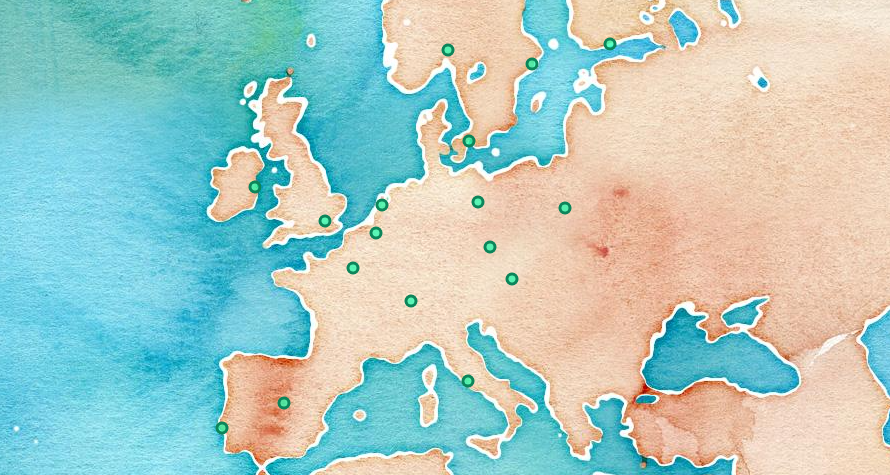
\includegraphics[width=\linewidth]{cities}
	\caption{Capital cities of Europe of interest to the client. }
	\label{fig:cities}
\end{figure}

\begin{table}[htbp!]
	\centering
	\caption{Obtained data for each country/capital.}
	\label{tab:data}
	\scalebox{0.85}{\begin{tabular}{llp{2.5cm}p{2.5cm}p{2.5cm}p{2.1cm}}
		\toprule
		\textbf{Country} 	& \textbf{Capital}  & \textbf{Percentage of vegetarians, \%} & \textbf{Percentage of vegans, \%} & \textbf{Number of vegetarian restaurants, -} & \textbf{Disposable income, \$} \\ \midrule
		Austria			& Vienna	& 10.0	& 2.8 & 	61 & 	32496 \\ 
		Belgium			& Brussels	& 7.0	& 1.0 & 	55 & 	29361 \\ 
		Czech Republic	& Prague	& 5.0	& 1.0 & 	70 & 	17984 \\ 
		Denmark			& Copenhagen& 10.0	& 4.0 & 	71 & 	28926 \\ 
		Finland			& Helsinki	& 11.0	& 2.0 & 	95 & 	26774 \\ 
		France			& Paris		& 5.2	& 1.1 & 	67 & 	25865 \\ 
		Germany			& Berlin	& 12.0	& 2.0 & 	57 & 	27569 \\ 
		Italy			& Rome		& 8.9	& 2.2 & 	36 & 	23023 \\ 
		Ireland			& Dublin	& 8.4	& 2.0 & 	47 & 	25933 \\ 
		Netherlands		& Amsterdam	& 5.0	& 1.0 & 	23 & 	29571 \\ 
		Norway			& Oslo		& 9.0	& 4.0 & 	19 & 	35542 \\ 
		Poland			& Warsaw	& 8.4	& 7.0 & 	23 & 	16507 \\ 
		Portugal		& Lisbon	& 1.2	& 0.6 & 	11 & 	15403 \\ 
		Spain			& Madrid	& 1.5	& 0.2 & 	62 & 	21788 \\ 
		Sweden			& Stockholm	& 12.0	& 4.0 & 	65 & 	29765 \\ 
		Switzerland		& Bern		& 5.0	& 1.0 & 	9  & 	37749 \\ 
		United Kingdom	& London	& 21.3	& 4.4 &    100 & 	22603 \\ 
		\bottomrule
	\end{tabular}}
\end{table}

\section{Methodology}
\label{sec:methodology}


\section{Results}
\label{sec:results}

\section{Discussion}
\label{sec:discussion}

\section{Conclusion}
\label{sec:conclusion}

\newpage
\appendix
\bibliographystyle{ieeetr} 
\bibliography{bib}


\end{document}          
